% Options for packages loaded elsewhere
\PassOptionsToPackage{unicode}{hyperref}
\PassOptionsToPackage{hyphens}{url}
%
\documentclass[
]{article}
\usepackage{lmodern}
\usepackage{amssymb,amsmath}
\usepackage{ifxetex,ifluatex}
\ifnum 0\ifxetex 1\fi\ifluatex 1\fi=0 % if pdftex
  \usepackage[T1]{fontenc}
  \usepackage[utf8]{inputenc}
  \usepackage{textcomp} % provide euro and other symbols
\else % if luatex or xetex
  \usepackage{unicode-math}
  \defaultfontfeatures{Scale=MatchLowercase}
  \defaultfontfeatures[\rmfamily]{Ligatures=TeX,Scale=1}
\fi
% Use upquote if available, for straight quotes in verbatim environments
\IfFileExists{upquote.sty}{\usepackage{upquote}}{}
\IfFileExists{microtype.sty}{% use microtype if available
  \usepackage[]{microtype}
  \UseMicrotypeSet[protrusion]{basicmath} % disable protrusion for tt fonts
}{}
\makeatletter
\@ifundefined{KOMAClassName}{% if non-KOMA class
  \IfFileExists{parskip.sty}{%
    \usepackage{parskip}
  }{% else
    \setlength{\parindent}{0pt}
    \setlength{\parskip}{6pt plus 2pt minus 1pt}}
}{% if KOMA class
  \KOMAoptions{parskip=half}}
\makeatother
\usepackage{xcolor}
\IfFileExists{xurl.sty}{\usepackage{xurl}}{} % add URL line breaks if available
\IfFileExists{bookmark.sty}{\usepackage{bookmark}}{\usepackage{hyperref}}
\hypersetup{
  pdftitle={Background},
  hidelinks,
  pdfcreator={LaTeX via pandoc}}
\urlstyle{same} % disable monospaced font for URLs
\usepackage[a4paper,margin=2cm]{geometry}
\usepackage{color}
\usepackage{fancyvrb}
\newcommand{\VerbBar}{|}
\newcommand{\VERB}{\Verb[commandchars=\\\{\}]}
\DefineVerbatimEnvironment{Highlighting}{Verbatim}{commandchars=\\\{\}}
% Add ',fontsize=\small' for more characters per line
\newenvironment{Shaded}{}{}
\newcommand{\AlertTok}[1]{\textcolor[rgb]{1.00,0.00,0.00}{\textbf{#1}}}
\newcommand{\AnnotationTok}[1]{\textcolor[rgb]{0.38,0.63,0.69}{\textbf{\textit{#1}}}}
\newcommand{\AttributeTok}[1]{\textcolor[rgb]{0.49,0.56,0.16}{#1}}
\newcommand{\BaseNTok}[1]{\textcolor[rgb]{0.25,0.63,0.44}{#1}}
\newcommand{\BuiltInTok}[1]{#1}
\newcommand{\CharTok}[1]{\textcolor[rgb]{0.25,0.44,0.63}{#1}}
\newcommand{\CommentTok}[1]{\textcolor[rgb]{0.38,0.63,0.69}{\textit{#1}}}
\newcommand{\CommentVarTok}[1]{\textcolor[rgb]{0.38,0.63,0.69}{\textbf{\textit{#1}}}}
\newcommand{\ConstantTok}[1]{\textcolor[rgb]{0.53,0.00,0.00}{#1}}
\newcommand{\ControlFlowTok}[1]{\textcolor[rgb]{0.00,0.44,0.13}{\textbf{#1}}}
\newcommand{\DataTypeTok}[1]{\textcolor[rgb]{0.56,0.13,0.00}{#1}}
\newcommand{\DecValTok}[1]{\textcolor[rgb]{0.25,0.63,0.44}{#1}}
\newcommand{\DocumentationTok}[1]{\textcolor[rgb]{0.73,0.13,0.13}{\textit{#1}}}
\newcommand{\ErrorTok}[1]{\textcolor[rgb]{1.00,0.00,0.00}{\textbf{#1}}}
\newcommand{\ExtensionTok}[1]{#1}
\newcommand{\FloatTok}[1]{\textcolor[rgb]{0.25,0.63,0.44}{#1}}
\newcommand{\FunctionTok}[1]{\textcolor[rgb]{0.02,0.16,0.49}{#1}}
\newcommand{\ImportTok}[1]{#1}
\newcommand{\InformationTok}[1]{\textcolor[rgb]{0.38,0.63,0.69}{\textbf{\textit{#1}}}}
\newcommand{\KeywordTok}[1]{\textcolor[rgb]{0.00,0.44,0.13}{\textbf{#1}}}
\newcommand{\NormalTok}[1]{#1}
\newcommand{\OperatorTok}[1]{\textcolor[rgb]{0.40,0.40,0.40}{#1}}
\newcommand{\OtherTok}[1]{\textcolor[rgb]{0.00,0.44,0.13}{#1}}
\newcommand{\PreprocessorTok}[1]{\textcolor[rgb]{0.74,0.48,0.00}{#1}}
\newcommand{\RegionMarkerTok}[1]{#1}
\newcommand{\SpecialCharTok}[1]{\textcolor[rgb]{0.25,0.44,0.63}{#1}}
\newcommand{\SpecialStringTok}[1]{\textcolor[rgb]{0.73,0.40,0.53}{#1}}
\newcommand{\StringTok}[1]{\textcolor[rgb]{0.25,0.44,0.63}{#1}}
\newcommand{\VariableTok}[1]{\textcolor[rgb]{0.10,0.09,0.49}{#1}}
\newcommand{\VerbatimStringTok}[1]{\textcolor[rgb]{0.25,0.44,0.63}{#1}}
\newcommand{\WarningTok}[1]{\textcolor[rgb]{0.38,0.63,0.69}{\textbf{\textit{#1}}}}
\usepackage{graphicx}
\makeatletter
\def\maxwidth{\ifdim\Gin@nat@width>\linewidth\linewidth\else\Gin@nat@width\fi}
\def\maxheight{\ifdim\Gin@nat@height>\textheight\textheight\else\Gin@nat@height\fi}
\makeatother
% Scale images if necessary, so that they will not overflow the page
% margins by default, and it is still possible to overwrite the defaults
% using explicit options in \includegraphics[width, height, ...]{}
\setkeys{Gin}{width=\maxwidth,height=\maxheight,keepaspectratio}
% Set default figure placement to htbp
\makeatletter
\def\fps@figure{htbp}
\makeatother
\setlength{\emergencystretch}{3em} % prevent overfull lines
\providecommand{\tightlist}{%
  \setlength{\itemsep}{0pt}\setlength{\parskip}{0pt}}
\setcounter{secnumdepth}{-\maxdimen} % remove section numbering
\usepackage{graphicx}
\usepackage{pgfplots}
\usepackage{hyperref}
\usepackage{tikz,tikz-3dplot} 
\usepackage{tkz-euclide}
\usetikzlibrary{arrows, automata}
\usepackage{fancyhdr}
\usepackage{float}
\usepackage{subcaption}
\pagestyle{fancy}
\usetikzlibrary{shapes.geometric}
\usetikzlibrary{calc}
\usetikzlibrary{angles}
\usepackage{setspace}
\usepackage[acronym]{glossaries-extra}
\setabbreviationstyle[acronym]{long-short}
\makeglossaries
\ifluatex
  \usepackage{selnolig}  % disable illegal ligatures
\fi

\title{Background}
\author{}
\date{}

\begin{document}
\maketitle

{
\setcounter{tocdepth}{3}
\tableofcontents
}
\newacronym{gr}{GR}{general relativity}
\newacronym{sr}{SR}{special relativity}
\newacronym{gps}{GPS}{Global Positition System}
\newacronym{bh}{BH}{black hole}
\newacronym{embedding}{embedding diagram}{embedding diagram}
\captionsetup{format=hang,indention=-0.5cm}
\onehalfspacing
\setlength{\parskip}{1.5em}

\hypertarget{background}{%
\section{Background}\label{background}}

\hypertarget{primer}{%
\subsection{A Primer on Spacetime and Relativity}\label{primer}}

\[\ \]

\pagebreak

\hypertarget{cartographer-design}{%
\subsection{Cartographer: Design}\label{cartographer-design}}

The Cartographer framework works by discretizing curved spacetime into a
lattice of vertices. The \texttt{Latticework} class is initialized by
specifying the interval and resolution for each spatial dimension. These
parameters are independent of each other and allow for optimization with
respect to computational runtime versus accuracy of the simulation. The
\texttt{Latticework} object then instantiates two NumPy arrays as a mesh
to represent the spacetime geometry.

At this stage, the lattice can be used to explore the underlying
geometry through the embedding diagrams in Section
\ref{#distanceTimeAndEmbedding}. To visualize motion, two \texttt{Stone}
objects are created with the initial conditions to be explored: energy
per unit mass, \(E/m\), and orbital angular momentum\footnote{Future
  references to angular momentum will omit the \emph{orbital} clarifier
  as spin angular momentum is not discussed or explored in this paper.}
per unit mass, \(L/m\). These objects are used as parameters for
calculating both their theoretical and simulated paths.

The \texttt{VerletPathfinding} class uses numerical integration with the
Verlet Velocity method (Section \ref{#verletAlgo}) to calculate the
theoretical geodesic and uses a time step size parameter for controlling
the accuracy of the path. The \texttt{Latticework} class uses the
\(A^*\) (``A star'') pathfinding algorithm (Section \ref{#astarAlgo})
and the principle of least action to determine how the stone should move
about the given geometry. A selection of helper data classes created to
aid in the readability and verbosity of the code are featured in
Appendix \ref{#helperClasses}.

\hypertarget{verletAlgo}{%
\subsubsection{Verlet Velocity Algorithm}\label{verletAlgo}}

The Verlet Velocity Algorithm approximates future position, velocity,
and acceleration by using two time steps of data to calculate the next
time step. This algorithm, like Euler's method, uses a Taylor series
expansion of the position function around a time \(t\) describing the
future position as

\begin{equation}\label{eqn:TaylorPosition}
x(t + \Delta t) = x(t) + \Delta t x^\prime (t) + \frac{(\Delta t)^2 x^{\prime\prime} (t)}{2} + \mathcal{O}(\Delta t^3).
\end{equation}

A simple Python implementation of Equation \ref{eqn:TaylorPosition}
typically looks like

\begin{Shaded}
\begin{Highlighting}[]
\NormalTok{dt, t, total\_time }\OperatorTok{=}\NormalTok{ ...}
\ControlFlowTok{while}\NormalTok{ t }\OperatorTok{\textless{}}\NormalTok{ total\_time:}
\NormalTok{    current\_acceleration }\OperatorTok{=}\NormalTok{ net\_force }\OperatorTok{/}\NormalTok{ mass}
\NormalTok{    current\_velocity }\OperatorTok{=}\NormalTok{ current\_velocity }\OperatorTok{+}\NormalTok{ current\_acceleration }\OperatorTok{*}\NormalTok{ dt}
\NormalTok{    current\_position }\OperatorTok{=}\NormalTok{ current\_position }\OperatorTok{+}\NormalTok{ current\_velocity}\OperatorTok{*}\NormalTok{dt}
\NormalTok{    t }\OperatorTok{=}\NormalTok{ t }\OperatorTok{+}\NormalTok{ dt}
\end{Highlighting}
\end{Shaded}

While both the Verlet Velocity and Euler's methods use the forward
difference definition for derivatives,

\begin{equation}
x^\prime (t) \approx \frac{x(t + \Delta t) - x(t)}{\Delta t},
\end{equation}

Euler's method only considers the derivatives and the position function
at \(t\) to inform the output for \(t+\Delta t\). The Verlet Velocity
method improves the accuracy by considering both expansions for
\(x(t+\Delta t)\) and \(x(t-\Delta t)\). \(x(t+\Delta t\) is then
reexpressed as the sum of the two expansions,

\begin{equation}
x(t+\Delta t) = 2x(t) - x(t-\Delta t) + \frac{(\Delta t)^2 a(t)}{2} + \mathcal{O}(\Delta t^4) .
\end{equation}

\hypertarget{astarAlgo}{%
\subsubsection{\texorpdfstring{\(A^*\) Pathfinding
Algorithm}{A\^{}* Pathfinding Algorithm}}\label{astarAlgo}}

The \(A^*\) search algorithm is a heuristic method for navigating
graphs. Two common applications for this type of algorithm are the
movement of units in a strategy computer game and a mobile GPS providing
directions. The problem is classified by considering a weighted graph of
nodes, such as in Figure \ref{fig:weightedGraph}. Each node represents
some intermediate destination along the way from a source to the desired
target. Each edge then has a real valued number corresponding to the
cost of moving to the next node.

\begin{figure}[H]
\centering
    \scalebox{0.95}{
        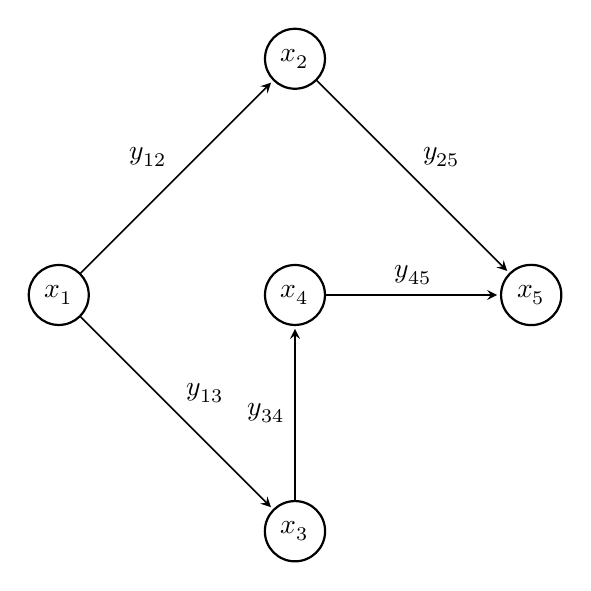
\begin{tikzpicture}[
                    > = stealth, % arrow head style
                    shorten > = 1pt, % don't touch arrow head to node
                    auto,
                    node distance = 3cm, % distance between nodes
                    semithick % line style
            ]

            \tikzstyle{every state}=[
                draw = black,
                thick,
                fill = white,
                minimum size = 4mm
            ]

            \node[state] (X1) {$x_1$};
            \node[state] (X4) [right of=X1] {$x_4$};
            \node[state] (X2) [above of=X4] {$x_2$};
            \node[state] (X3) [below of=X4] {$x_3$};
            \node[state] (X5) [right of=X4] {$x_5$};
            
            \draw[-stealth] (X1) -- (X2) node[midway] {$y_{12}$};
            \draw[-stealth] (X1) -- (X3) node[midway] {$y_{13}$};
            \draw[-stealth] (X2) -- (X5) node[midway] {$y_{25}$};
            \draw[-stealth] (X3) -- (X4) node[midway] {$y_{34}$};
            \draw[-stealth] (X4) -- (X5) node[midway] {$y_{45}$};
        \end{tikzpicture}
    }
    \caption{In this directed graph, each $x_i$ is a node and each $y_{ij}$ represents the cost to traverse from $x_i$ to $x_j$. For this example, there are two possible paths from the source node $x_1$ to $x_5$: (1) $x_1 \rightarrow x_2 \rightarrow x_5$ and (2) $x_1 \rightarrow x_3 \rightarrow x_4 \rightarrow x_5$ with total respective costs of $y_{12}+y_{25}$ and $y_{13}+y_{34}+y_{45}$. }
    \label{fig:weightedGraph}
\end{figure}

While the example shown in Figure \ref{fig:weightedGraph} is simplistic,
the underlying heuristic of \(A^*\) will not increase in complexity as
the weight graph increases. The algorithm walks through the graph by
visiting each node and recording the cost to reach each neighboring
node. Once the target node has been reached, the algorithm then sorts
through all possible paths by the smallest total cost. Figure
\ref{fig:WeightGraph2} represents the same structure but with numeric
values for the costs, which allows for a definitive answer to ``what is
the shortest path from \(x_1\) to \(x_5\)?''

\begin{figure}[H]
    \begin{subfigure}{0.9\textwidth}
    \centering
    \scalebox{0.8}{
        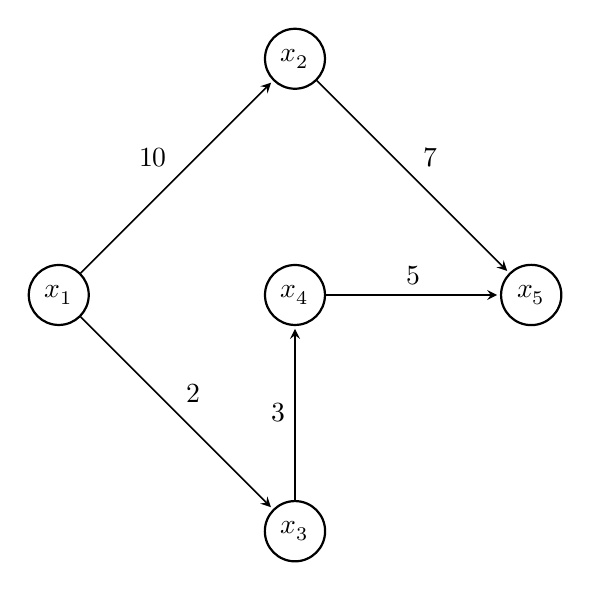
\begin{tikzpicture}[
                > = stealth, % arrow head style
                shorten > = 1pt, % don't touch arrow head to node
                auto,
                node distance = 3cm, % distance between nodes
                semithick % line style
        ]

        \tikzstyle{every state}=[
            draw = black,
            thick,
            fill = white,
            minimum size = 4mm
        ]

        \node[state] (X1) {$x_1$};
        \node[state] (X4) [right of=X1] {$x_4$};
        \node[state] (X2) [above of=X4] {$x_2$};
        \node[state] (X3) [below of=X4] {$x_3$};
        \node[state] (X5) [right of=X4] {$x_5$};
        
        \draw[-stealth] (X1) -- (X2) node[midway] {$10$};
        \draw[-stealth] (X1) -- (X3) node[midway] {$2$};
        \draw[-stealth] (X2) -- (X5) node[midway] {$7$};
        \draw[-stealth] (X3) -- (X4) node[midway] {$3$};
        \draw[-stealth] (X4) -- (X5) node[midway] {$5$};

        \end{tikzpicture}
    }
    \end{subfigure}
    \newline
    \begin{subfigure}{0.45\textwidth}
    \centering
    \scalebox{0.75}{
        \begin{tikzpicture}[
                > = stealth, % arrow head style
                shorten > = 1pt, % don't touch arrow head to node
                auto,
                node distance = 3cm, % distance between nodes
                semithick % line style
        ]

        \tikzstyle{every state}=[
            draw = black,
            thick,
            fill = white,
            minimum size = 4mm
        ]

        \node[state] (X1) [below left of=X2{$x_1$};
        \node[state] (X2) {$x_2$};
        \node[state] (X5) [below right of=X2] {$x_5$};
        
        \draw[-stealth] (X1) -- (X2) node[midway] {$10$};
        \draw[-stealth] (X2) -- (X5) node[midway] {$7$};

        \end{tikzpicture}
    }
    \end{subfigure}
    \hfill
    \begin{subfigure}{0.45\textwidth}
    \centering
    \scalebox{0.75}{
        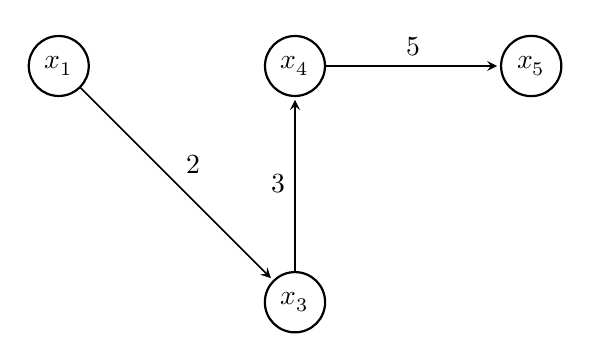
\begin{tikzpicture}[
                > = stealth, % arrow head style
                shorten > = 1pt, % don't touch arrow head to node
                auto,
                node distance = 3cm, % distance between nodes
                semithick % line style
        ]

        \tikzstyle{every state}=[
            draw = black,
            thick,
            fill = white,
            minimum size = 4mm
        ]

        \node[state] (X1) {$x_1$};
        \node[state] (X4) [right of=X1] {$x_4$};
        \node[state] (X3) [below of=X4] {$x_3$};
        \node[state] (X5) [right of=X4] {$x_5$};
        
        \draw[-stealth] (X1) -- (X3) node[midway] {$2$};
        \draw[-stealth] (X3) -- (X4) node[midway] {$3$};
        \draw[-stealth] (X4) -- (X5) node[midway] {$5$};

        \end{tikzpicture}   
    }
    \end{subfigure}
    \caption{While the first path, $x_1 \rightarrow x_2 \rightarrow x_5$, has fewer edges traversed, the total cost of this path is $17$, whereas the other path, $x_1 \rightarrow x_3 \rightarrow x_4 \rightarrow x_5$, visits more nodes but has a total cost of $10$.}
    \label{fig:WeightGraph2}
\end{figure}

To increase readability of the code, a series of helper data classes
were created to allow clear descriptions and the intended use of each
parameter.

is easily controlled by specifying the parameters in the
\texttt{Dimension} data class. The size and resolution of each spatial
dimension is controlled by specifying the corresponding parameters in
the \texttt{dimensions} data class. The resolution (or spacing between
each vertex) for each dimension is independent of each other, allowing
for explicit control of the density of nodes. All information specific
to the geometry of the given spacetime is stored inside the
\texttt{latticework} object.

In order to increase readability, an object-oriented design approach
used in the creation of Cartographer. The key feature of using OOP for
this, is that responsibilities and actions are delegated to specific
objects which allows for the code to self-narrate what is being done and
reduce the scope of variables. For this purpose, several helper data
classes and objects were created: \texttt{Coordinate}, \texttt{Stone},
and \texttt{Latticework}.

The \texttt{Coordinate} class accepts either a pair of spatial cartesian
coordinates, \(x\) and \(y\), or polar coordinates, \(r\) and \(\phi\).
In connection with the coordinate system discussed in Section
\ref{primer}, either representation corresponds to the Bookkeeper's
coordinate system (e.g.~\(r\) is the reduced circumference
`\(r\)-coordinate'). Instances of \texttt{Coordinate} also have access
to two functions that return either the \texttt{Cartesian} or
\texttt{Polar} data classes to allow easy transition between coordinate
systems. The other notable property is that each \texttt{Coordinate}
calculates and provides access to the curvature for its location, either
by direct computation from

\begin{minipage}{0.15\textwidth}
    \raggedright
    \begin{verbatim}example_coordinate.curvature\end{verbatim}
\end{minipage}
\begin{minipage}{0.8\textwidth}
    \begin{equation}
        = 1-\frac{2M}{r}
    \end{equation}
\end{minipage}

or by

\begin{minipage}{0.15\textwidth}
    \raggedright
    \begin{verbatim}example_coordinate.curvature\end{verbatim}
\end{minipage}
\begin{minipage}{0.8\textwidth}
    \begin{equation}
        = 1-\frac{2M}{\sqrt{x^2 + y^2}}.
    \end{equation}
\end{minipage}

The \texttt{Stone} class acts as the container for all information of
the low-mass/massless object that will be traversing the curved
spacetime. There's a beautiful symmetry here in that all initial
conditions for the physical object are stored by instance representing
that object. As a result, the \texttt{Stone} class is fairly empty, only
containing a record of its previous positions, energy per unit mass
(\(E/m\)), and angular momentum per unit mass (\(L/m\)). All of the
instructions about how to move through the geometry are given externally
through \texttt{Latticework} as the curvature dictates or by numerical
integration.

\texttt{Latticework} takes the parameters specified by the
\texttt{Dimension} instance and creates a 2-dimensional NumPy mesh grid.

\end{document}
